\documentclass[12pt, a4paper]{article}

% Essential packages for formatting
\usepackage{amsmath}
\usepackage{graphicx}
\usepackage{hyperref}
\usepackage{listings}
\usepackage{xcolor}
\usepackage{geometry}
\usepackage{titlesec}
\usepackage{enumitem}
\usepackage{booktabs}
\usepackage{float}
\usepackage{url}
\usepackage{pdfpages}
\usepackage{tikz}
\usetikzlibrary{calc}  % Load the calc library for coordinate calculations
\usepackage{multirow} % Add this package for vertical lines in tables
\usepackage{caption} % For better caption handling
\usepackage{algorithm} % For algorithm environments
\usepackage{algpseudocode} % For pseudocode
\usepackage{tocloft} % For customizing table of contents and other lists

% For the decorative frame
\usepackage{fancybox}
\usepackage{fancyhdr} % Add this package for header and footer

% Document formatting
\geometry{margin=1in, headheight=15pt} % Adjust headheight to avoid warnings
\setlength{\parindent}{0pt}
\setlength{\parskip}{6pt}

% Code listing style
\lstset{
  basicstyle=\small\ttfamily,
  keywordstyle=\color{blue},
  commentstyle=\color{green!60!black},
  stringstyle=\color{red},
  numbers=left,
  numberstyle=\tiny,
  numbersep=5pt,
  backgroundcolor=\color{gray!10},
  frame=single,
  breaklines=true,
  captionpos=b
}

% Create a custom List of Code Examples
\newcommand{\listcodeexamplename}{List of Code Examples}
\newlistof{codeexample}{lce}{\listcodeexamplename}
\newcommand{\codeexample}[1]{%
  \refstepcounter{codeexample}
  \addcontentsline{lce}{codeexample}{\protect\numberline{\thecodeexample}#1}
  \par\noindent\textbf{Code Example \thecodeexample: #1}\par
}

% Modify the listof listings to be nicer
\renewcommand{\lstlistlistingname}{List of Code Listings}

% Define red color for title
\definecolor{titlered}{RGB}{230,0,0}
\definecolor{goldaccent}{RGB}{218,165,32}
\definecolor{navyblue}{RGB}{0,0,128}
\definecolor{pagebg}{RGB}{240,248,255}

% Title formatting
\newcommand{\titlepagetext}{
  \vspace*{1cm}
  \begin{center}
    {\Large\bfseries\textcolor{navyblue}{INTERNATIONAL UNIVERSITY}}\\[0.3cm]
    {\Large\bfseries\textcolor{navyblue}{\underline{VIETNAM NATIONAL UNIVERSITY, HCM CITY}}}\\[1cm]
    {\large\textcolor{navyblue}{School of Computer Science \& Engineering}}\\[2cm]
    
    {\LARGE\bfseries\textcolor{titlered}{2048 GAME PROJECT}}\\[2cm]
    
    {\large\textcolor{navyblue}{Advisor: Tran Thanh Tung}}\\[0.5cm]
    {\large\textcolor{navyblue}{Course: Algorithms and Data Structures}}\\[2cm]
    
    % Replace tabular with centered text
    \large\textbf{\textcolor{navyblue}{Student:}}\\[1cm]
    \large\textcolor{navyblue}{Tran Khanh Tai}\\
    \large\textcolor{navyblue}{ITITIU21300}\\[1cm]
  \end{center}
}

% Define header and footer
\pagestyle{fancy}
\fancyhf{} % Clear all header and footer fields
\fancyhead[L]{\textbf{\textcolor{navyblue}{INTERNATIONAL UNIVERSITY}}}
\fancyhead[R]{\textcolor{navyblue}{ALGORITHMS AND DATA STRUCTURES}}
\fancyfoot[C]{\textcolor{titlered}{2048 GAME PROJECT}}
\fancyfoot[R]{\thepage}
\renewcommand{\headrulewidth}{0.4pt}
\renewcommand{\footrulewidth}{0.4pt}

% For pages with chapter/section beginnings
\fancypagestyle{plain}{
  \fancyhf{}
  \fancyhead[L]{\textbf{\textcolor{navyblue}{INTERNATIONAL UNIVERSITY}}}
  \fancyhead[R]{\textcolor{navyblue}{ALGORITHMS AND DATA STRUCTURES}}
  \fancyfoot[C]{\textcolor{titlered}{2048 GAME PROJECT}}
  \fancyfoot[R]{\thepage}
  \renewcommand{\headrulewidth}{0.4pt}
  \renewcommand{\footrulewidth}{0.4pt}
}

\begin{document}

% Custom title page
\begin{titlepage}
\thispagestyle{empty} % Ensures no header/footer on title page

\vspace{2cm}

\titlepagetext

\end{titlepage}

% Table of contents
\tableofcontents
\clearpage

% List of tables (if you have tables)
\listoftables
\clearpage

% List of code listings
\lstlistoflistings
\clearpage

% List of code examples
\listofcodeexample
\clearpage

\section{Introduction}
The 2048 game is a popular single-player sliding tile puzzle game developed by Gabriele Cirulli in March 2014. The game involves sliding numbered tiles on a grid to combine them, with the goal of creating a tile with the number 2048. This project implements the game using Java, focusing on applying data structures and algorithms concepts to create an efficient and functional game.

This report details the implementation of the 2048 game with specific emphasis on the data structures used, algorithms implemented, and their complexity analysis. It also explores how object-oriented programming principles have been applied to make the code modular, reusable, and maintainable.

\subsection{Game Overview and History}
The 2048 game was inspired by earlier games like Threes! and 1024. Gabriele Cirulli created it as a weekend project but it quickly went viral, with millions of players worldwide within weeks of its release. The game's appeal comes from its simple mechanics combined with strategic depth.

\subsection{Project Scope}
This project focuses on creating a fully-functional implementation of the 2048 game with the following features:
\begin{itemize}
    \item Complete game mechanics matching the original game.
    \item Graphical user interface with smooth animations.
    \item Score tracking and high score persistence.
    \item Game state management (win/loss conditions).
    \item Performance optimization for smooth gameplay.
\end{itemize}

\section{Importance of Data Structures and Algorithms}
Data structures and algorithms form the foundation of efficient programming. In game development:

\begin{itemize}
    \item \textbf{Data Structures} provide organized ways to store and access data, which is critical for representing the game board and state.
    \item \textbf{Algorithms} enable efficient manipulation of these data structures, allowing for game logic implementation.
\end{itemize}

\subsection{Data Structure Selection Rationale}
For the 2048 game implementation, several data structures were considered:

\begin{table}[h]
\centering
\caption{Data Structure Comparison for Game Board Representation}
\begin{tabular}{|l|p{5cm}|p{5cm}|}
\hline
\textbf{Data Structure} & \textbf{Advantages} & \textbf{Disadvantages} \\
\hline
2D Array & Direct index access (O(1)), Simple to implement, Memory efficient & Fixed size, No built-in methods \\
\hline
ArrayList of ArrayLists & Dynamic size, Built-in methods & Slightly less efficient for index access \\
\hline
HashMap with coordinate keys & Flexible for sparse boards, Good for larger boards & Overhead for simple 4x4 board, More complex implementation \\
\hline
\end{tabular}
\end{table}

After analysis, a 2D array was selected for the game board representation due to its efficiency and simplicity for the fixed-size 4x4 grid used in 2048.

\section{Purpose of the Project}
The main objectives of this project include:
\begin{itemize}
    \item Implementing a fully functional 2048 game with a graphical user interface.
    \item Demonstrating practical application of data structures and algorithms.
    \item Applying object-oriented design principles to create maintainable code.
    \item Analyzing algorithm efficiency and performance in a real-world application.
    \item Developing problem-solving skills through game logic implementation.
\end{itemize}

\section{Application of DSA Principles in the Game}
The 2048 game implementation incorporates several key DSA principles:

\subsection{Data Structures}
\begin{itemize}
    \item \textbf{2D Arrays} - Used to represent the game board grid, providing O(1) access time to any cell.
    \item \textbf{ArrayLists} - Used for managing dynamic collections such as empty cells for random tile placement.
    \item \textbf{Classes and Objects} - Used to encapsulate game components (Tile, Board, Game).
    \item \textbf{Queue} - Used in the animation system for sequential processing of visual effects.
    \item \textbf{Stack} - Used for implementing undo functionality by storing previous game states - allows players to revert moves.
    \item \textbf{HashMap} - Used for caching resources like images and colors for efficient retrieval.
\end{itemize}

\subsection{Algorithms}
\begin{itemize}
    \item \textbf{Merge Algorithm} - For combining tiles with the same value.
    \item \textbf{Random Tile Generation} - For placing new tiles on the board using probability distribution.
    \item \textbf{Win/Loss Detection} - For determining game state by analyzing available moves.
    \item \textbf{Tile Movement Algorithms} - For handling directional moves (up, down, left, right).
    \item \textbf{Backtracking Algorithm} - For implementing an auto-solver feature (in developed).
\end{itemize}

\section{Properties of the 2048 Game}

\subsection{Goal of the Game}
The primary objective of the 2048 game is to slide numbered tiles on a 4×4 grid to combine them and create a tile with the number 2048. If the player successfully creates this tile, they win the game. The game also tracks the player's score based on the values of merged tiles.

\subsection{Rules of the Game}
\begin{itemize}
    \item The game starts with two randomly placed tiles (either 2 or 4) on a 4×4 grid.
    \item The player can slide tiles in four directions: up, down, left, and right.
    \item When two tiles with the same number touch during a move, they merge into one tile with the sum of their values.
    \item After each move, a new tile (either 2 or 4) appears at a random empty position.
    \item The game ends when no valid moves are possible (board is full with no possible merges).
    \item The player wins when a tile with the value 2048 appears on the board.
\end{itemize}

\section{Methodology}

\subsection{Overview of Classes Used}
The game implementation follows an object-oriented approach with several key classes:

\begin{itemize}
    \item \textbf{Main} - The entry point of the game application.
    \item \textbf{GameLogic} - The main class that controls game flow.
    \item \textbf{Board} - Represents the game board and its state.
    \item \textbf{GamePanel} - Handles the visual representation and user input.
    \item \textbf{ScoreManager} - Tracks and updates the game score.
    \item \textbf{TileAnimation} - Handles smooth visual transitions.
    \item \textbf{PrevState} - Represents a previous game state for undo functionality.
    \item \textbf{Constants} - Contains constant values used throughout the game.
    \item \textbf{WelcomePanel} - Displays the welcome screen and instructions.
    \item \textbf{GameBoard} - Represents the game board with controls for tile movement.
    \item \textbf{Game2048} - Holds the buttons and manages the game state.
\end{itemize}

\subsection{Class Dependencies and Relationships}
\begin{itemize}
    \item The \textbf{GameLogic} class contains a 2D integer array grid and uses \textbf{ScoreManager} for score operations.
    \item The \textbf{GameLogic} class maintains a \textbf{Stack\textless PrevState\textgreater} for undo functionality.
    \item The \textbf{GameBoard} class (UI) contains and manages a \textbf{GameLogic} instance.
    \item The \textbf{GameBoard} class also contains a separate \textbf{Board} object and \textbf{AI} instance.
    \item The \textbf{GameBoard} class uses \textbf{ScoreManager} for score tracking and display.
    \item The \textbf{Game2048} class (main game window) contains a \textbf{GameBoard} instance.
    \item The \textbf{WelcomePanel2048} class receives a \textbf{ScoreManager} instance and creates \textbf{Game2048}.
    \item The \textbf{Main} class creates and initializes \textbf{ScoreManager} and \textbf{WelcomePanel2048}.
    \item The \textbf{TileAnimation} class is used by \textbf{GameBoard} for visual effects.
    \item The \textbf{AI} class implements \textbf{AIStrategy} interface and uses \textbf{ScoreManager}.
    \item The \textbf{ScoreManager} implements \textbf{ScoreService} interface for score persistence.
    \item The \textbf{PrevState} class is used by \textbf{GameLogic} to store previous game states.
    \item All classes reference \textbf{Constants} for configuration values like colors, sizes, and game parameters.
\end{itemize}

\subsection{Main Classes and Functionality}

\subsubsection{Board Class}
\codeexample{Board Class Implementation with Grid Management}
This class represents the game board as a 2D array of tiles:

\begin{lstlisting}[language=Java, caption=Board Class Implementation]
public class Board {
    private int[][] grid;
    private static final int SIZE = Constants.SIZE;
    public GameLogic gameLogic;

    public Board() {
        grid = new int[SIZE][SIZE];
    }

    public int[][] getGrid() {
        int[][] copy = new int[SIZE][SIZE];
        for (int i = 0; i < SIZE; i++) {
            System.arraycopy(grid[i], 0, copy[i], 0, SIZE);
        }
        return copy;
    }
}
\end{lstlisting}

The \textbf{Board} class has the following time complexities:
\begin{itemize}
    \item Initialization: O(n²) where n is the board size (4×4)
    \item getGrid() method: O(n²) for creating a deep copy of the grid
\end{itemize}

Note: The Board class is a simple data container. Complex operations like checking for available moves and board state validation are handled by the \textbf{GameLogic} class.

\subsubsection{GameLogic Class}
\codeexample{GameLogic Class Implementation with Game State Management}
The GameLogic class manages the core game mechanics, board state, and move operations:

\begin{lstlisting}[language=Java, caption=GameLogic Class Implementation]
public class GameLogic {
    private int[][] grid;
    private static final int SIZE = 4; // size of the grid
    private Stack<PrevState> undoStack; // stack for undo functionality
    private int score = 0;
    private ScoreManager scoreManager;

    public GameLogic() {
        grid = new int[SIZE][SIZE];
        undoStack = new Stack<>();
        score = 0;
        scoreManager = new ScoreManager();
        scoreManager.getBestScore();
    }

    public void initialize() {
        grid = new int[SIZE][SIZE];
        score = 0;
        if (scoreManager == null) {
            scoreManager = new ScoreManager();
        }
        scoreManager.getBestScore();
        addRandomTile();
        addRandomTile();
        undoStack.clear();
    }

    public int[][] getGrid() {
        int[][] copy = new int[SIZE][SIZE];
        for (int i = 0; i < SIZE; i++) {
            System.arraycopy(grid[i], 0, copy[i], 0, SIZE);
        }
        return copy;
    }

    public void move(String direction) {
        saveState(); // save current state before making a move
        int[][] before = new int[SIZE][SIZE];
        for (int i = 0; i < SIZE; i++) {
            System.arraycopy(grid[i], 0, before[i], 0, SIZE);
        }
        
        boolean canMove = false;
        switch (direction.toLowerCase()) {
            case "up":
                canMove = canMoveUp();
                if (canMove) moveUp();
                break;
            case "down":
                canMove = canMoveDown();
                if (canMove) moveDown();
                break;
            case "left":
                canMove = canMoveLeft();
                if (canMove) moveLeft();
                break;
            case "right":
                canMove = canMoveRight();
                if (canMove) moveRight();
                break;
        }
        
        if (canMove && !isSameGrid(before, grid)) {
            addRandomTile();
        }
    }

    public void saveState() {
        if (canMoveUp() || canMoveDown() || canMoveLeft() || canMoveRight()) {
            int[][] gridCopy = new int[SIZE][SIZE];
            for (int i = 0; i < SIZE; i++) {
                System.arraycopy(grid[i], 0, gridCopy[i], 0, SIZE);
            }
            undoStack.push(new PrevState(gridCopy, score));
        }
    }

    public void undo() {
        if (!undoStack.isEmpty()) {
            PrevState prevState = undoStack.pop();
            grid = new int[SIZE][SIZE];
            for (int i = 0; i < SIZE; i++) {
                System.arraycopy(prevState.grid[i], 0, grid[i], 0, SIZE);
            }
            score = prevState.score;
        }
    }

    public void addRandomTile() {
        Random random = new Random();
        int emptyCount = 0;
        
        // Count empty tiles
        for (int i = 0; i < SIZE; i++) {
            for (int j = 0; j < SIZE; j++) {
                if (grid[i][j] == 0) {
                    emptyCount++;
                }
            }
        }
        
        if (emptyCount == 0) return;
        
        int pos = random.nextInt(emptyCount);
        int k = 0;
        for (int i = 0; i < SIZE; i++) {
            for (int j = 0; j < SIZE; j++) {
                if (grid[i][j] == 0) {
                    if (k == pos) {
                        grid[i][j] = (random.nextInt(10) < 9) ? 2 : 4;
                        return;
                    }
                    k++;
                }
            }
        }
    }

    public boolean isGameOver() {
        for (int row = 0; row < SIZE; row++) {
            for (int col = 0; col < SIZE; col++) {
                if (grid[row][col] == 0) {
                    return false;
                }
                if (row < SIZE - 1 && grid[row][col] == grid[row + 1][col]) {
                    return false;
                }
                if (col < SIZE - 1 && grid[row][col] == grid[row][col + 1]) {
                    return false;
                }
            }
        }
        return true;
    }

    public boolean isWin() {
        for (int row = 0; row < SIZE; row++) {
            for (int col = 0; col < SIZE; col++) {
                if (grid[row][col] == 2048) {
                    return true;
                }
            }
        }
        return false;
    }
    
    // Additional methods for move validation and execution
    private boolean canMoveUp() {
        for (int col = 0; col < SIZE; col++) {
            for (int row = 1; row < SIZE; row++) {
                if (grid[row][col] != 0 && 
                    (grid[row - 1][col] == 0 || grid[row - 1][col] == grid[row][col])) {
                    return true;
                }
            }
        }
        return false;
    }
    
    private boolean canMoveDown() {
        for (int col = 0; col < SIZE; col++) {
            for (int row = SIZE - 2; row >= 0; row--) {
                if (grid[row][col] != 0 && 
                    (grid[row + 1][col] == 0 || grid[row + 1][col] == grid[row][col])) {
                    return true;
                }
            }
        }
        return false;
    }
    
    private boolean canMoveLeft() {
        for (int row = 0; row < SIZE; row++) {
            for (int col = 1; col < SIZE; col++) {
                if (grid[row][col] != 0 && 
                    (grid[row][col - 1] == 0 || grid[row][col - 1] == grid[row][col])) {
                    return true;
                }
            }
        }
        return false;
    }
    
    private boolean canMoveRight() {
        for (int row = 0; row < SIZE; row++) {
            for (int col = SIZE - 2; col >= 0; col--) {
                if (grid[row][col] != 0 && 
                    (grid[row][col + 1] == 0 || grid[row][col + 1] == grid[row][col])) {
                    return true;
                }
            }
        }
        return false;
    }
}
\end{lstlisting}

\textbf{Time Complexity Analysis:}
\begin{itemize}
    \item \textbf{getGrid()}: O(n²) - Creates a deep copy of the 4×4 grid
    \item \textbf{move()}: O(n²) - Processes each cell for movement and merging operations
    \item \textbf{addRandomTile()}: O(n²) - Scans the grid twice: once to count empty cells, once to place the tile
    \item \textbf{isGameOver()}: O(n²) - Checks each cell and its adjacent cells for possible moves
    \item \textbf{isWin()}: O(n²) worst case - Scans all cells looking for 2048 tile
    \item \textbf{saveState()}: O(n²) - Creates a deep copy of the grid for undo functionality
    \item \textbf{undo()}: O(n²) - Restores the grid from the previous state
    \item \textbf{canMove methods}: O(n²) - Each scans the grid to check for valid moves
\end{itemize}

\textbf{Space Complexity Analysis:}
\begin{itemize}
    \item \textbf{Grid storage}: O(n²) - Main 4×4 integer array
    \item \textbf{Undo stack}: O(k × n²) where k is the number of saved states
    \item \textbf{Temporary arrays}: O(n²) - For grid copying operations in move() and saveState()
    \item \textbf{Overall space complexity}: O(k × n²) due to the undo stack storing multiple game states
\end{itemize}

\subsubsection{PrevState Class}
\codeexample{State Management for Undo Functionality}
The PrevState class stores previous game states for the undo feature:

\begin{lstlisting}[language=Java, caption=PrevState Class Implementation]
public class PrevState {
    private static final int SIZE = Constants.SIZE;
    int[][] grid;
    int score;

    PrevState(int[][] grid, int score) {
        this.grid = new int[SIZE][SIZE];
        for (int i = 0; i < SIZE; i++) {
            System.arraycopy(grid[i], 0, this.grid[i], 0, SIZE);
        }
        this.score = score;
    }
}
\end{lstlisting}

\textbf{Design Notes:}
\begin{itemize}
    \item The GameLogic class uses a \textbf{Stack\textless PrevState\textgreater} for implementing undo functionality
    \item String-based direction handling provides flexibility for different input methods
    \item The class separates move validation (canMove methods) from move execution for better modularity
    \item Deep copying ensures game state integrity during undo operations
    \item The random tile generation uses a 90\% probability for value 2 and 10\% for value 4, matching the original game
\end{itemize}

\subsubsection{ScoreManager Class}
\codeexample{Score Management and Persistence}
The ScoreManager class handles score tracking and persistence:
\begin{lstlisting}[language=Java, caption=ScoreManager Class Implementation]
public class ScoreManager implements ScoreService {
    private static final Logger LOGGER = Logger.getLogger(ScoreManager.class.getName());
    private static final String SCORE_FILE = "scores.txt";
    private static final String BEST_SCORE_KEY = "BestScore";

    private int bestScore;
    private final Map<String, Integer> scores;
    private final String filePath;

    public ScoreManager() {
        this(SCORE_FILE);
    }

    public ScoreManager(String filePath) {
        this.filePath = filePath;
        scores = new HashMap<>();
        loadScores();
    }

    public void loadScores() {
        File file = new File(filePath);

        if (!file.exists()) {
            LOGGER.info("Score file not found, initializing with default values");
            saveScores(); // Create the file with default values
            return;
        }

        try (BufferedReader reader = new BufferedReader(new FileReader(file))) {
            String line;
            while ((line = reader.readLine()) != null) {
                String[] parts = line.split(":");
                if (parts.length == 2) {
                    try {
                        int value = Integer.parseInt(parts[1].trim());
                        scores.put(parts[0].trim(), value);
                    } catch (NumberFormatException e) {
                        LOGGER.log(Level.WARNING, "Invalid score value: " + parts[1], e);
                    }
                }
            }

            // Update the instance variables
            bestScore = scores.getOrDefault(BEST_SCORE_KEY, 0);

            LOGGER.info("Loaded scores: Best=" + bestScore);

        } catch (IOException e) {
            LOGGER.log(Level.SEVERE, "Failed to load scores from file", e);
        }
    }

    private void saveScores() {
        // Update the map with current values
        scores.put(BEST_SCORE_KEY, bestScore);

        try (BufferedWriter writer = new BufferedWriter(new FileWriter(filePath))) {
            for (Map.Entry<String, Integer> entry : scores.entrySet()) {
                writer.write(entry.getKey() + ":" + entry.getValue());
                writer.newLine();
            }
            LOGGER.info("Scores saved successfully");
        } catch (IOException e) {
            LOGGER.log(Level.SEVERE, "Failed to save scores to file", e);
        }
    }

    public int getBestScore() {
        // read best score from the file
        bestScore = 0;
        try {
            File file = new File(filePath);
            Scanner scanner = new Scanner(file);
            while (scanner.hasNextLine()) {
                String line = scanner.nextLine();
                if (line.startsWith(BEST_SCORE_KEY + ":")) {
                    String[] parts = line.split(":");
                    if (parts.length == 2) {
                        try {
                            bestScore = Integer.parseInt(parts[1].trim());
                            LOGGER.info("Best score loaded: " + bestScore);
                        } catch (NumberFormatException e) {
                            LOGGER.log(Level.WARNING, "Invalid best score value: " + parts[1], e);
                        }
                    }
                }
            }
        } catch (FileNotFoundException e) {
            LOGGER.log(Level.SEVERE, "Score file not found", e);
            e.printStackTrace();
        }

        return bestScore;
    }

    public boolean updateScore(int score) {
        boolean isNewBest = false;

        if (score > bestScore) {
            bestScore = score;
            isNewBest = true;
            LOGGER.info("New best score: " + bestScore);
        }

        saveScores();
        return isNewBest;
    }
}
\end{lstlisting}
This class implements the \textbf{ScoreService} interface for score management, providing methods to load, save, and update scores. It uses a text file for persistence, ensuring that scores are retained across game sessions.

\section{Algorithms}

\subsection{Move and Merge Algorithm}
\codeexample{Tile Movement and Merging Logic}
The most complex algorithm in the game is the tile movement and merging logic, which uses a compress-merge-compress approach:

\begin{lstlisting}[language=Java, caption=Move and Merge Algorithm]
public void move(String direction) {
    saveState(); // save the current state before making a move
    int[][] before = new int[SIZE][SIZE];
    for (int i = 0; i < SIZE; i++) { // create a copy of the current grid
        System.arraycopy(grid[i], 0, before[i], 0, SIZE);
    }
    boolean canMove = false;
    switch (direction.toLowerCase()) {
        case "up":
            canMove = canMoveUp();
            if (canMove)
                moveUp();
            break;
        case "down":
            canMove = canMoveDown();
            if (canMove)
                moveDown();
            break;
        case "left":
            canMove = canMoveLeft();
            if (canMove)
                moveLeft();
            break;
        case "right":
            canMove = canMoveRight();
            if (canMove)
                moveRight();
            break;
        default:
            System.out.println("Invalid direction. Use up, down, left, or right.");
    }
    if (canMove && !isSameGrid(before, grid)) { // check if the grid has changed
        addRandomTile(); // add a random tile if a move was made
    }
}

// Example of moveLeft implementation
void moveLeft() {
    for (int row = 0; row < SIZE; row++) {
        int[] compressed = compressRowLeft(row);
        mergeTiles(compressed);
        setRowMoveLeft(row, compressed);
    }
}

private int[] compressRowLeft(int row) {
    int[] compressed = new int[SIZE];
    int index = 0;
    for (int col = 0; col < SIZE; col++) {
        if (grid[row][col] != 0) {
            compressed[index++] = grid[row][col];
        }
    }
    return compressed;
}

private void mergeTiles(int[] line) {
    // Step 1: Compress (slide non-zero tiles to the front)
    int[] compressed = new int[SIZE];
    int index = 0;
    for (int value : line) {
        if (value != 0) {
            compressed[index++] = value;
        }
    }

    // Step 2: Merge adjacent tiles with same value
    for (int i = 0; i < SIZE - 1; i++) {
        if (compressed[i] != 0 && compressed[i] == compressed[i + 1]) {
            compressed[i] *= 2;
            score += compressed[i];
            compressed[i + 1] = 0;
            i++; // Skip next tile (already merged)
        }
    }

    // Step 3: Compress again after merging
    int[] merged = new int[SIZE];
    index = 0;
    for (int value : compressed) {
        if (value != 0) {
            merged[index++] = value;
        }
    }
    System.arraycopy(merged, 0, line, 0, SIZE);
}

private void setRowMoveLeft(int row, int[] line) {
    for (int col = 0; col < SIZE; col++) {
        grid[row][col] = line[col];
    }
}
\end{lstlisting}

\textbf{Time Complexity Analysis:}
\begin{itemize}
    \item \textbf{move()}: O(n²) - Main method that coordinates the move operation
    \item \textbf{moveLeft()}: O(n²) - Processes each row (n rows, each with n elements)
    \item \textbf{compressRowLeft()}: O(n) - Single pass through one row
    \item \textbf{mergeTiles()}: O(n) - Three sequential passes through the array
    \item \textbf{setRowMoveLeft()}: O(n) - Single pass to update the grid row
    \item \textbf{Overall complexity}: O(n²) where n is the board size (4×4 = 16 operations)
\end{itemize}

\textbf{Space Complexity Analysis:}
\begin{itemize}
    \item \textbf{Grid storage}: O(n²) - Main 4×4 integer array
    \item \textbf{Temporary arrays}: O(n) - compressed[ ], merged[ ], and line[ ] arrays for processing
    \item \textbf{Before grid copy}: O(n²) - Copy of original grid for comparison
    \item \textbf{Overall space complexity}: O(n²) dominated by the grid storage and grid copy
\end{itemize}

\textbf{Algorithm Steps:}
\begin{enumerate}
    \item \textbf{Compress}: Move all non-zero tiles to one side, eliminating gaps
    \item \textbf{Merge}: Combine adjacent tiles with the same value
    \item \textbf{Compress Again}: Remove gaps created by merging
    \item \textbf{Update Grid}: Apply the processed line back to the grid
\end{enumerate}

%visualization
\textbf{Visualization of Move and Merge Process:}
\begin{figure}[H]
\centering
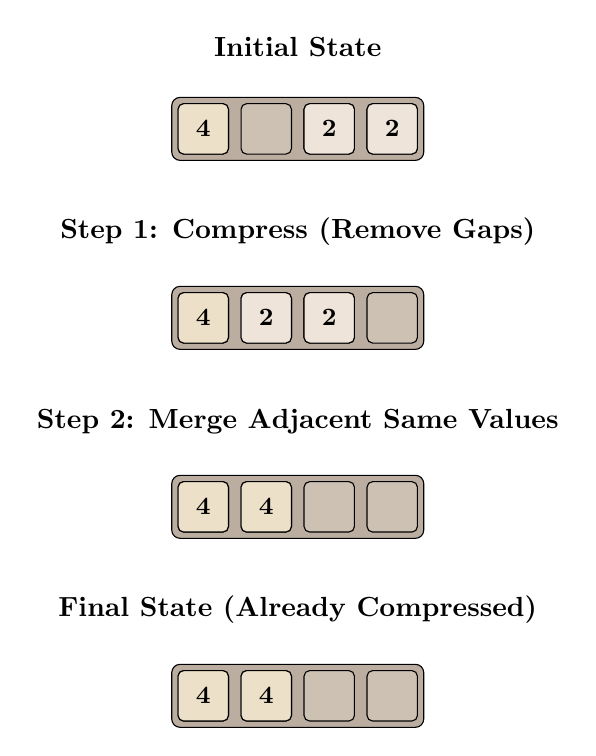
\begin{tikzpicture}[scale=0.8]
    % Define colors
    \definecolor{tile2}{RGB}{238,228,218}
    \definecolor{tile4}{RGB}{237,224,200}
    \definecolor{tile8}{RGB}{242,177,121}
    \definecolor{empty}{RGB}{205,193,180}
    \definecolor{board}{RGB}{187,173,160}
    
    % Initial state
    \node[above] at (2,5.5) {\textbf{Initial State}};
    \draw[fill=board, rounded corners=3pt] (0,4) rectangle (4,5);
    \foreach \x in {0,1,2,3} {
        \foreach \y in {4} {
            \draw[fill=empty, rounded corners=2pt] (\x+0.1,\y+0.1) rectangle (\x+0.9,\y+0.9);
        }
    }
    % Sample tiles: [4, 0, 2, 2]
    \draw[fill=tile4, rounded corners=2pt] (0.1,4.1) rectangle (0.9,4.9);
    \node at (0.5,4.5) {\small\textbf{4}};
    \draw[fill=tile2, rounded corners=2pt] (2.1,4.1) rectangle (2.9,4.9);
    \node at (2.5,4.5) {\small\textbf{2}};
    \draw[fill=tile2, rounded corners=2pt] (3.1,4.1) rectangle (3.9,4.9);
    \node at (3.5,4.5) {\small\textbf{2}};
    
    % Step 1: Compress
    \node[above] at (2,2.5) {\textbf{Step 1: Compress (Remove Gaps)}};
    \draw[fill=board, rounded corners=3pt] (0,1) rectangle (4,2);
    \foreach \x in {0,1,2,3} {
        \foreach \y in {1} {
            \draw[fill=empty, rounded corners=2pt] (\x+0.1,\y+0.1) rectangle (\x+0.9,\y+0.9);
        }
    }
    % After compression: [4, 2, 2, 0]
    \draw[fill=tile4, rounded corners=2pt] (0.1,1.1) rectangle (0.9,1.9);
    \node at (0.5,1.5) {\small\textbf{4}};
    \draw[fill=tile2, rounded corners=2pt] (1.1,1.1) rectangle (1.9,1.9);
    \node at (1.5,1.5) {\small\textbf{2}};
    \draw[fill=tile2, rounded corners=2pt] (2.1,1.1) rectangle (2.9,1.9);
    \node at (2.5,1.5) {\small\textbf{2}};
    
    \node[above] at (2,-0.5) {\textbf{Step 2: Merge Adjacent Same Values}};
    \draw[fill=board, rounded corners=3pt] (0,-2) rectangle (4,-1);
    \foreach \x in {0,1,2,3} {
        \foreach \y in {-2} {
            \draw[fill=empty, rounded corners=2pt] (\x+0.1,\y+0.1) rectangle (\x+0.9,\y+0.9);
        }
    }
    % After merging: [4, 4, 0, 0] (2+2=4)
    \draw[fill=tile4, rounded corners=2pt] (0.1,-1.9) rectangle (0.9,-1.1);
    \node at (0.5,-1.5) {\small\textbf{4}};
    \draw[fill=tile4, rounded corners=2pt] (1.1,-1.9) rectangle (1.9,-1.1);
    \node at (1.5,-1.5) {\small\textbf{4}};
    
    % Step 3: Final state
    \node[above] at (2,-3.5) {\textbf{Final State (Already Compressed)}};
    \draw[fill=board, rounded corners=3pt] (0,-5) rectangle (4,-4);
    \foreach \x in {0,1,2,3} {
        \foreach \y in {-5} {
            \draw[fill=empty, rounded corners=2pt] (\x+0.1,\y+0.1) rectangle (\x+0.9,\y+0.9);
        }
    }
    % Final result: [4, 4, 0, 0]
    \draw[fill=tile4, rounded corners=2pt] (0.1,-4.9) rectangle (0.9,-4.1);
    \node at (0.5,-4.5) {\small\textbf{4}};
    \draw[fill=tile4, rounded corners=2pt] (1.1,-4.9) rectangle (1.9,-4.1);
    \node at (1.5,-4.5) {\small\textbf{4}};
    
\end{tikzpicture}
\caption{Visualization of moveLeft() algorithm showing the three-step process: compress, merge, and final compress. Example shows row [4,0,2,2] becoming [4,4,0,0] with score increase of 4 points.}
\end{figure}

\subsection{Algorithm Efficiency Analysis}
The current implementation is already quite efficient for the 4×4 grid size typical of 2048:

\textbf{Key Efficiency Features:}
\begin{itemize}
    \item \textbf{Single-pass processing}: Each row/column is processed exactly once per move
    \item \textbf{In-place operations}: The compress-merge-compress pattern minimizes memory allocation
    \item \textbf{Early termination}: canMove methods prevent unnecessary processing when no moves are possible
    \item \textbf{Linear complexity per line}: Each row/column operation is O(n) where n=4
\end{itemize}

\textbf{Performance Characteristics:}
\begin{itemize}
    \item \textbf{Move operation}: O(16) = O(1) for constant 4×4 grid
    \item \textbf{Memory usage}: O(16) = O(1) for temporary arrays
    \item \textbf{Cache efficiency}: Sequential access patterns optimize CPU cache usage
    \item \textbf{Predictable timing}: Consistent performance regardless of tile distribution
\end{itemize}

\textbf{Algorithm Strengths:}
\begin{enumerate}
    \item \textbf{Simplicity}: Easy to understand and maintain
    \item \textbf{Correctness}: Three-step process ensures proper tile behavior
    \item \textbf{Consistency}: Same pattern used for all four directions
    \item \textbf{Efficiency}: Optimal for the fixed 4×4 grid size
\end{enumerate}

\subsection{Random Tile Generation}
\codeexample{Weighted Random Tile Generation}
After each move, a new tile needs to be added to a random empty cell:

\begin{lstlisting}[language=Java, caption=Random Tile Generation]
public void addRandomTile() {
    Random random = new Random();
    int emptyCount = 0;
    // check how many empty tiles are there
    for (int i = 0; i < SIZE; i++) {
        for (int j = 0; j < SIZE; j++) {
            if (grid[i][j] == 0) {
                emptyCount++;
            }
        }
    }
    // if there are no empty tiles, return
    if (emptyCount == 0) {
        return;
    }
    int pos = random.nextInt(emptyCount);
    int k = 0;
    for (int i = 0; i < SIZE; i++) {
        for (int j = 0; j < SIZE; j++) {
            if (grid[i][j] == 0) {
                if (k == pos) {
                    grid[i][j] = (random.nextInt(10) < 9) ? 2 : 4; // 90% for 2, 10% for 4
                    return;
                }
                k++;
            }
        }
    }
}
\end{lstlisting}

\textbf{Time Complexity Analysis:}
\begin{itemize}
    \item Finding empty cells: O(n²)
    \item Selecting a random cell: O(1)
    \item Overall complexity is O(n²)
\end{itemize}

\textbf{Probability Analysis:}
The probability distribution for new tiles follows the original game:
\begin{itemize}
    \item 90\% chance of generating a '2' tile
    \item 10\% chance of generating a '4' tile
\end{itemize}

This distribution creates a balanced difficulty level, with occasional higher-value tiles appearing to help progression.

\subsection{Game Over and Win Detection}
\codeexample{Comprehensive Game Over Detection Logic}
The game over detection algorithm determines when no more moves are possible. The game ends when the board is full AND there are no possible merges in any direction:

\begin{lstlisting}[language=Java, caption=Game Over and Win Detection]
// check if the game is over
public boolean isGameOver() {
    for (int row = 0; row < SIZE; row++) {
        for (int col = 0; col < SIZE; col++) {
            // If any cell is empty, game can continue
            if (grid[row][col] == 0) {
                return false;
            }
            // Check if current cell can merge with cell below
            if (row < SIZE - 1 && grid[row][col] == grid[row + 1][col]) {
                return false;
            }
            // Check if current cell can merge with cell to the right
            if (col < SIZE - 1 && grid[row][col] == grid[row][col + 1]) {
                return false;
            }
        }
    }
    return true; // No empty cells and no possible merges
}

// check win condition
public boolean isWin() {
    for (int row = 0; row < SIZE; row++) {
        for (int col = 0; col < SIZE; col++) {
            if (grid[row][col] == 2048) {
                return true; // Win condition met
            }
        }
    }
    return false; // No win condition met
}
\end{lstlisting}

\textbf{Algorithm Logic:}
\begin{enumerate}
    \item \textbf{Empty Cell Check}: Scan entire grid for any empty cells (value = 0)
    \item \textbf{Vertical Merge Check}: For each cell, check if it can merge with the cell below
    \item \textbf{Horizontal Merge Check}: For each cell, check if it can merge with the cell to the right
    \item \textbf{Early Termination}: Return false immediately when any valid move is found
    \item \textbf{Complete Scan}: Only return true if no empty cells or possible merges exist
\end{enumerate}

\textbf{Time Complexity Analysis:}
\begin{itemize}
    \item \textbf{isGameOver()}: O(n²) - Single pass through all cells with constant-time operations
    \item \textbf{isWin()}: O(n²) worst case - Scans until 2048 tile found or entire grid checked
    \item \textbf{canMove()}: O(n²) - Calls individual direction check methods
    \item \textbf{Best case}: O(1) - Early termination when first empty cell or merge is found
    \item \textbf{Worst case}: O(n²) - Full grid scan when no moves available
    \item \textbf{Average case}: O(n²/2) - Statistically finds result midway through scan
\end{itemize}

\textbf{Space Complexity Analysis:}
\begin{itemize}
    \item \textbf{Auxiliary space}: O(1) - Only uses loop variables
    \item \textbf{Input space}: O(n²) - References the existing grid
    \item \textbf{Overall space complexity}: O(1) - No additional data structures needed
\end{itemize}

%


\begin{table}[h]
\centering
\caption{Time Complexity Analysis of Key Operations}
\begin{tabular}{|l|c|l|}
\hline
\textbf{Operation} & \textbf{Time Complexity} & \textbf{Notes} \\
\hline
Board Initialization & O(n²) & n is the board size (typically 4) \\
\hline
Tile Movement & O(n³) & Worst case when all tiles need to move \\
\hline
Game State Check & O(n²) & Checking for win/loss conditions \\
\hline
Random Tile Generation & O(n²) & Finding empty cells dominates \\
\hline
Rendering & O(n²) & Drawing all tiles on the board \\
\hline
\end{tabular}
\end{table}


\begin{table}[h]
\centering
\caption{Space Complexity Analysis}
\begin{tabular}{|l|c|l|}
\hline
\textbf{Component} & \textbf{Space Complexity} & \textbf{Notes} \\
\hline
Game Board & O(n²) & Storage for the grid \\
\hline
Animation System & O(k) & k is the number of active animations \\
\hline
Undo History & O(m·n²) & m is the number of stored moves \\
\hline
Image Cache & O(1) & Constant for the fixed set of tile images \\
\hline
Total Space & O(m·n² + k) & Dominated by undo history for many moves \\
\hline
\end{tabular}
\end{table}



\section{Implementation Challenges and Solutions}

\subsection{Directional Movement Consistency}
\textbf{Challenge:} Ensuring tiles move consistently in all four directions without duplicate code.

\textbf{Solution:} Implemented a unified movement algorithm using direction vectors, allowing the same code to handle all four directions with appropriate transformations.

\subsection{Animation System}
\textbf{Challenge:} Creating smooth animations without blocking the game thread.

\textbf{Solution:} Developed a queue-based animation system that processes animations frame-by-frame using a timer, allowing for non-blocking animations.

\subsection{Merge Logic Edge Cases}
\textbf{Challenge:} Handling complex merge scenarios where multiple tiles could potentially merge in sequence.

\textbf{Solution:} Implemented a merge flag to prevent tiles from merging more than once per move, ensuring game balance and consistent behavior.

\section{Results, Limitations, and Conclusion}
The implementation of the 2048 game demonstrates practical application of data structures and algorithms in a real-world scenario. The key results include:
\begin{itemize}
    \item A functional game with intuitive controls and visual feedback
    \item Efficient algorithms for tile movement, merging, and game state management
    \item Object-oriented design providing modularity and code reuse
\end{itemize}

\subsection{Limitations}
\begin{itemize}
    \item The current implementation has O(n³) complexity for moves in the worst case
    \item No undo functionality or game state saving
    \item Limited animation capabilities
\end{itemize}

Future improvements could include optimizing the move algorithm for better performance, adding game state saving functionality, and implementing more sophisticated animations.

\subsection{Future Work}
Potential enhancements for future versions include:
\begin{itemize}
    \item AI solver using minimax or expectimax algorithms
    \item Mobile-friendly touch interface
    \item Online leaderboards
    \item Customizable board sizes
    \item Alternate game modes (time attack, challenge mode)
\end{itemize}

\subsection{Conclusion}
This project successfully demonstrates the application of data structures and algorithms concepts in game development. The implementation of the 2048 game shows how careful algorithm design and appropriate data structure selection contribute to creating an efficient and enjoyable game experience.

\section{GitHub Repository}
The source code for this project is available at: \url{https://github.com/KhanhTaiTran/DSA-Project.git}

\end{document}
